\subsection{Milestones and Deliverables}

\pro milestones and deliverables will be along the following lines:

% Overall expenses related to personnel and equipment for a 4 year term
% of project development, testing and initial deployment in
% \ref{fig:expense}. The overall proportion of the costs in
% \ref{fig:exp-pie}

% \begin{table}[!h]
%   \centering
%   \vspace{-0.5cm}
%   \begin{tabular}{|p{1.8cm}|p{13cm}|}\hline 
%     \rowcolor{Gray}
%     \bfseries Year &\bfseries Description \\
%     \hline
%     \textbf{Sept/Oct 2021} & Proof-of-concept field demonstration off of
%                              Portugal, with assimilation of measurements from aerial, surface and
%                              underwater vehicles into oceanographic models with remote sensing
%                              provided by a \nas \sml overflight and other sources.\\  
%     \hline
%     \textbf{1} & Architectural system design with a focus on software
%                  integration, building hardware and design and testing of Machine
%                  Learning for ocean model prediction.\\ 
%     \hline
%     \textbf{1--2} & Use and integration of existing remote sensing data products
%                     (from \esa and \nase), integration of ocean models and building of
%                     AI-based adaptive control systems for aerial, surface and underwater
%                     vehicles. \\  
%     \hline
%     \textbf{1--2} & Incremental demonstration of closing the
%                     prediction-sensing-assimilation loop for dynamic ocean events in the
%                     coastal region.\\
%     \hline
%     \textbf{1--3} & Incremental at-sea testing of adaptations of robotic vehicles
%                     and integration of control with ocean model predictions.\\

%     \hline
%     \textbf{1--3} & Demonstrations of the integrative software system using existing
%                     aerial, surface and underwater vehicles and targeting a single
%                     use-case (e.g. from aquaculture, oil \& gas, others) for
%                     monetization.\\
%     \hline
%     \textbf{3--4} & Upscope demonstration to include larger data sources for
%                     physical ocean properties, including
%                     from buoys and surf forecasts.\\ 

%     \hline
%     \textbf{3--4} & Pursue European Union and other sources to fund a constellation
%                     of \smle's to demonstrate the full capability in a coastal ecosystem.\\ 
%     \hline
%   \end{tabular}
%   \caption{Proposed timeline of milestones and deliverables.}
%   \label{tab:timeline}
%   \vspace{-0.5cm}
% \end{table}

\begin{itemize}[noitemsep,topsep=0pt,parsep=5pt,partopsep=10pt]

\item A Sept/Oct 2021 proof-of-concept field demonstration off of
  Portugal, with assimilation of measurements from aerial, surface and
  underwater vehicles into oceanographic models with remote sensing
  provided by a cubesat that was developed with funding from the Moore
  Foundation as well as other more traditional sources.

\item Architectural system design with a focus on software
  integration, building hardware and design and testing of Machine
  Learning for ocean model prediction (Year \textbf{1})

\item Use and integration of existing remote sensing data products
  (from \esa and \nase), integration of ocean models and building of
  AI-based adaptive control systems for aerial, surface and underwater
  vehicles.  (Years \textbf{1--2})

\item Phased demonstration of closing the
  prediction-sensing-assimilation loop for dynamic ocean events in the
  coastal region (Years \textbf{1--2})

\item Phased at-sea testing of adaptations of robotic vehicles and
  integration of control with ocean model predictions (Years
  \textbf{1--3})

\item Demonstrations of the integrative software system using existing
  aerial, surface and underwater vehicles and targeting a single
  use-case (e.g. from aquaculture, oil \& gas, coastal pollution
  around urban centers, others) for monetization (Year \textbf{1--3})

\item Upscope demonstration to include larger data sources for
  physical ocean properties, including from buoys and surf forecasts
  (Years \textbf{3--4})

% \item \sml launch and operation begins. Validation of satellite
%   payloads and calibration of sensor performance (Years \textbf{4--5})

\item Pursue European Union and other sources to fund a constellation
  of \smle s to demonstrate the full capability in a coastal ecosystem
  (Years \textbf{3--4})
  
\end{itemize}

\begin{figure}[!t]
  \centering
  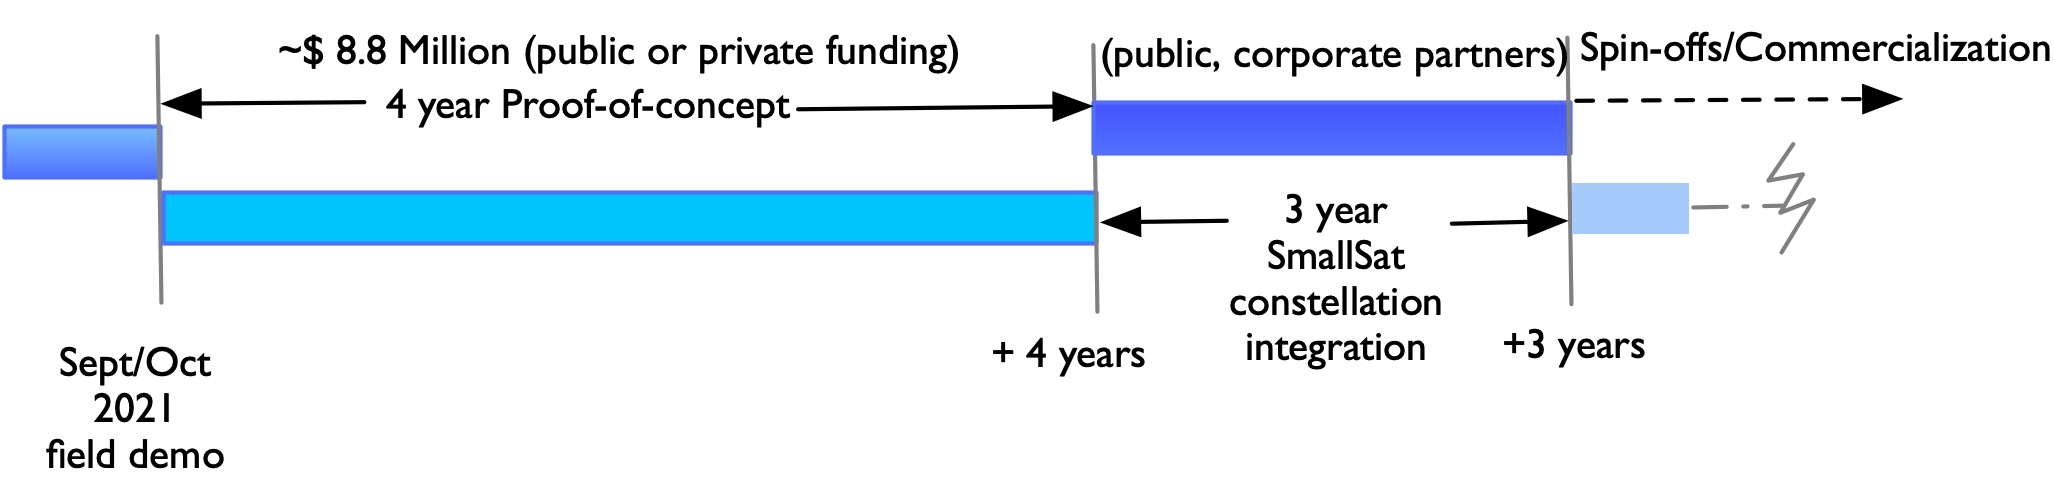
\includegraphics[scale=0.22]{fig/timeline.jpg}
  \caption{Overview of timeline in steps for \proe. Initial
    demonstration of key concepts with a simple demonstration in a
    field experiment in 2021 would ideally be followed by a systematic
    engineering effort to build the needed software
    infrastructure. Should \sml constellation build/test/launch/flight
    and purchase of hardware be possible, that effort can be
    accommodated with the software build shown.}
  \label{fig:timeline}
\end{figure}

% \noindent
Our first step will be a rapid and simple demonstration of the key
concepts in the September/October 2021 timeframe using existing remote
sensing products including that from an ocean color cubesat funded by
the Moore Foundation for environmental assimilation, and available
robotic platforms, for an experiment that links in-situ measurements
with ocean model assimilation, prediction and intelligent adaptive
sampling. We will use this exercise to demonstrate to key stakeholders
the potential of systematic integration of platforms and sensors, with
models, so as to visualize in detail, generated data products. A more
systematic integration, the focus of this proposal, will require the 4
year effort proposed above. Should sponsorship of the \sml
constellation occur during this phase, the build/test/launch/flight
and integration of these assets with the software will
commence. Subsequent spin-offs and commercialization will need skilled
staff to do the outreach to a range of commercial, governmental and
NGO entities.


% \begin{wrapfigure}{r}{0.45\textwidth}
%   % \vspace{-1cm}
%   \centering
%   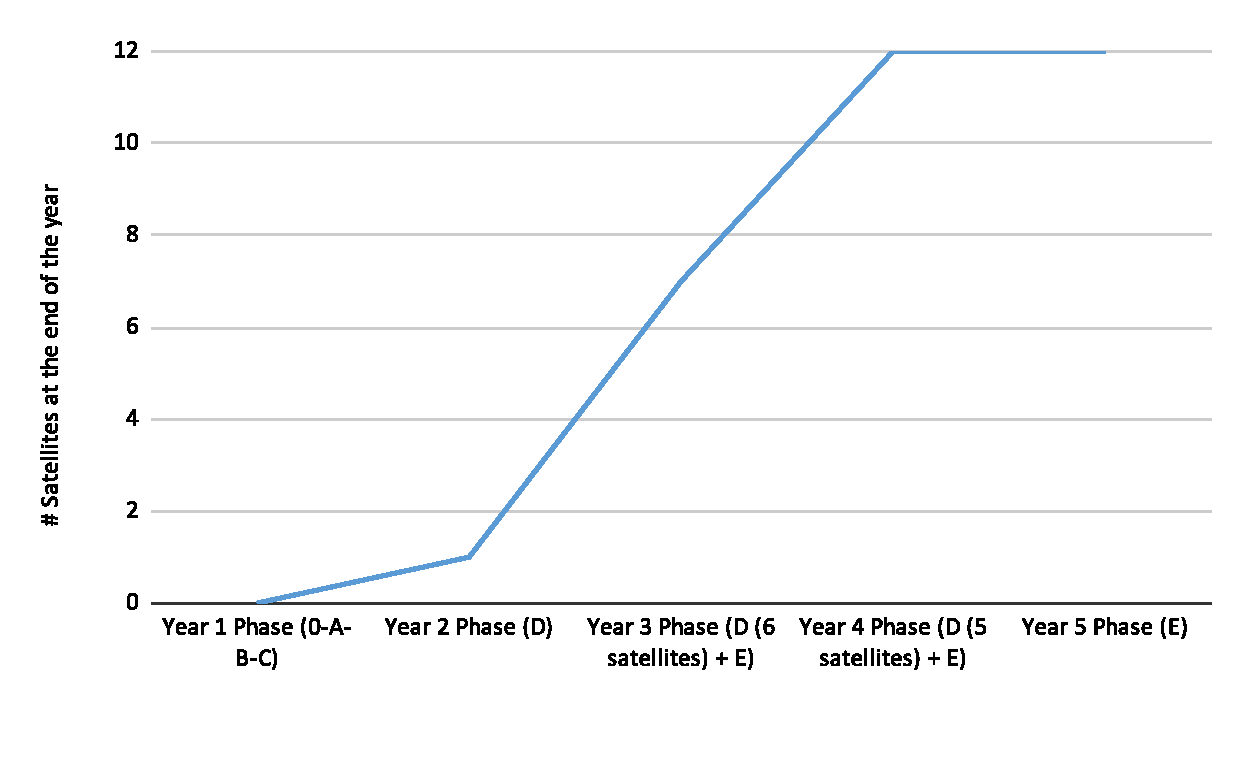
\includegraphics[scale=0.35]{fig/sat-progression.pdf}
%   \caption{Progression of deployment for 12 \smle's over a period of 5
%     years.}
%   \label{fig:sat-prog}
%   % \vspace{-0.5cm}
% \end{wrapfigure}


% shows costs associated with the project broken
% down to provide a clear picture of the distributions of proposed
% expenses. The end product will be a software system which will predict
% oceanographic conditions, use the prediction to adaptively place
% in-situ robotic vehicles to sample at the 'right place and right
% time', assimilate the sensed environment in ocean models and provide a
% reiterated prediction.

% Should the \sml part of the project be simultaneously
% executed with the development of software and hardware for in-situ
% assets, the two figures would then be merged. The incremental
% deployment of the \smle's is shown in Fig. \ref{fig:sat-prog}.

% \parbox[t]{\dimexpr\textwidth-\leftmargin}{%
%       \vspace{-2.5mm}
%       \begin{wrapfigure}[10]{r}{0.5\textwidth}
%         \centering
%         \vspace{-\baselineskip}
%         \subfigure[]{\label{fig:insitu}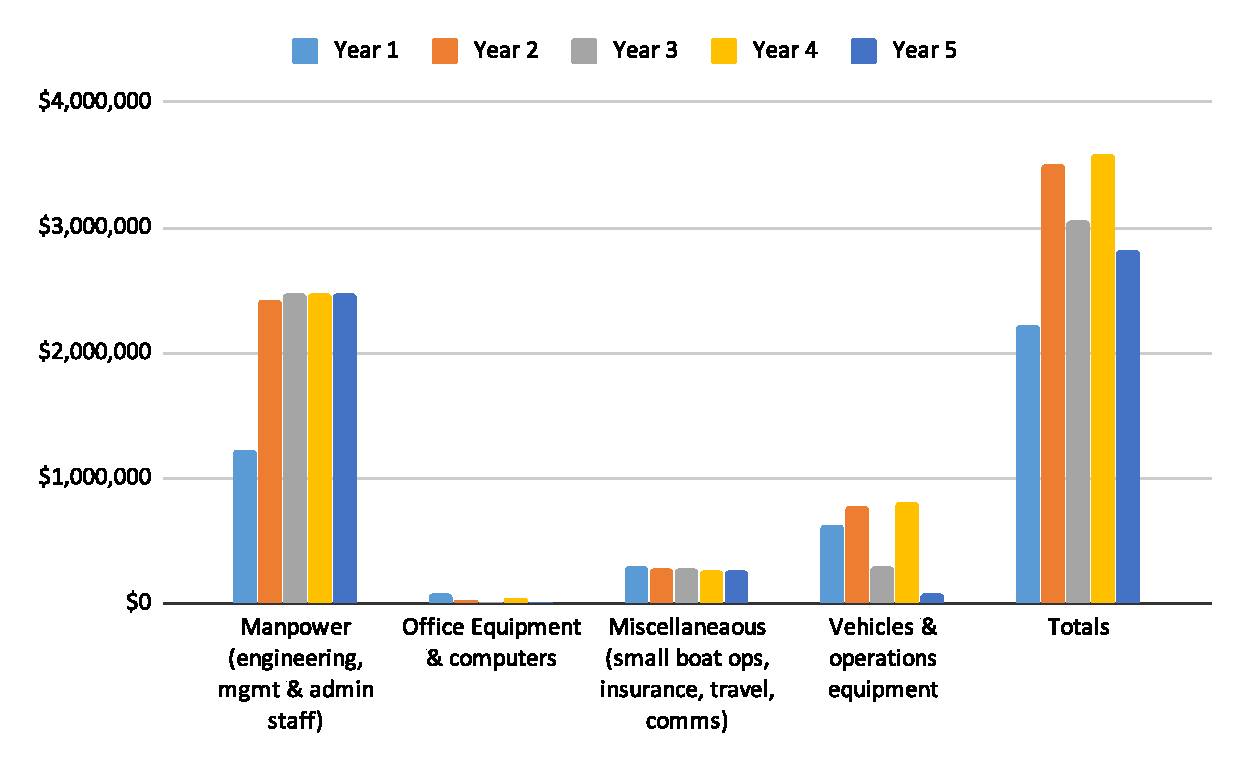
\includegraphics[width=.75\linewidth]{fig/insitu.pdf}}
%         \subfigure[]{\label{fig:sats}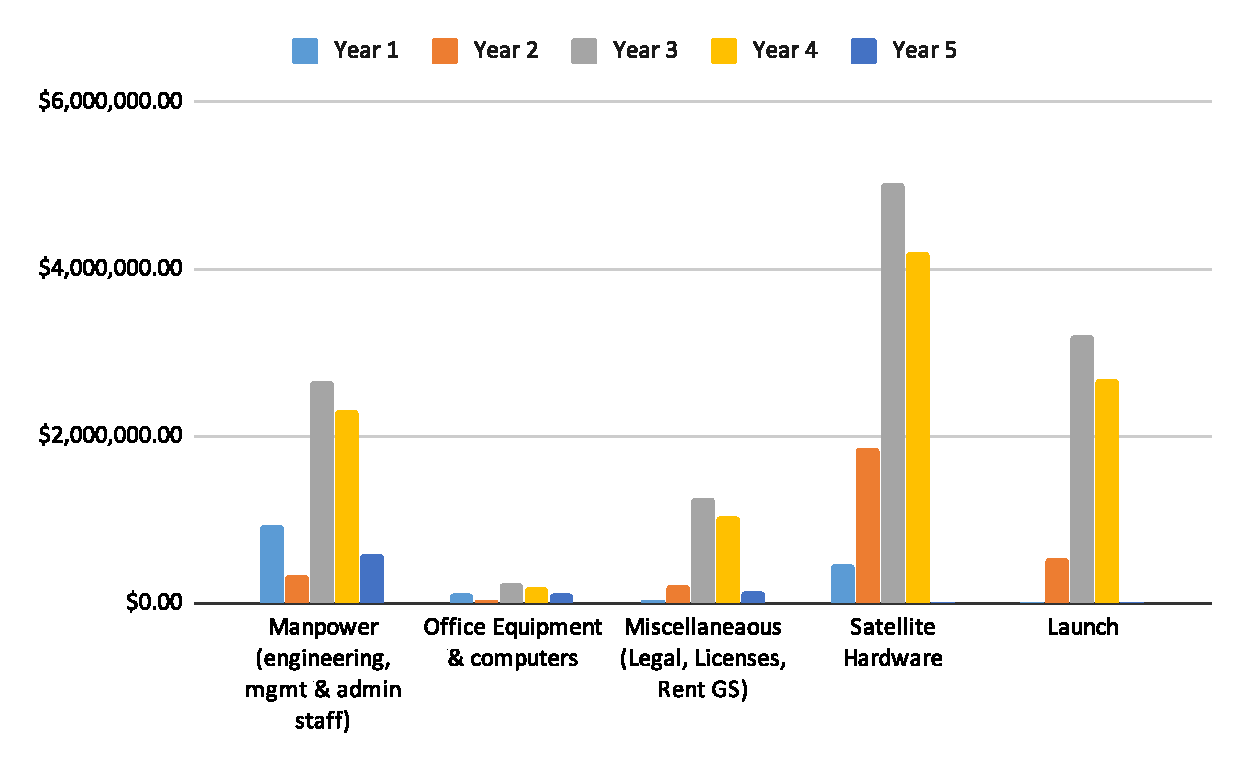
\includegraphics[width=.75\linewidth]{fig/sats.pdf}}
%         \caption{Costs and distribution for \ref{fig:insitu} assets and
%           software and \ref{fig:sats} \smle's over a 5 year project term.}
%       \end{wrapfigure}
%     }

% \noindent
Fig. \ref{fig:costs} shows the anticipated cost breakdown to provide a
clear picture of the distribution of the budget. The end product will
be a software system that will predict oceanographic conditions, use
the prediction to adaptively place in-situ robotic vehicles to take
water samples at the ‘right place and right time’, assimilate the
sensed environment in ocean models and provide a reiterated
prediction. 

\begin{figure}[!h]
  \centering
  \subfigure[]{\label{fig:expense}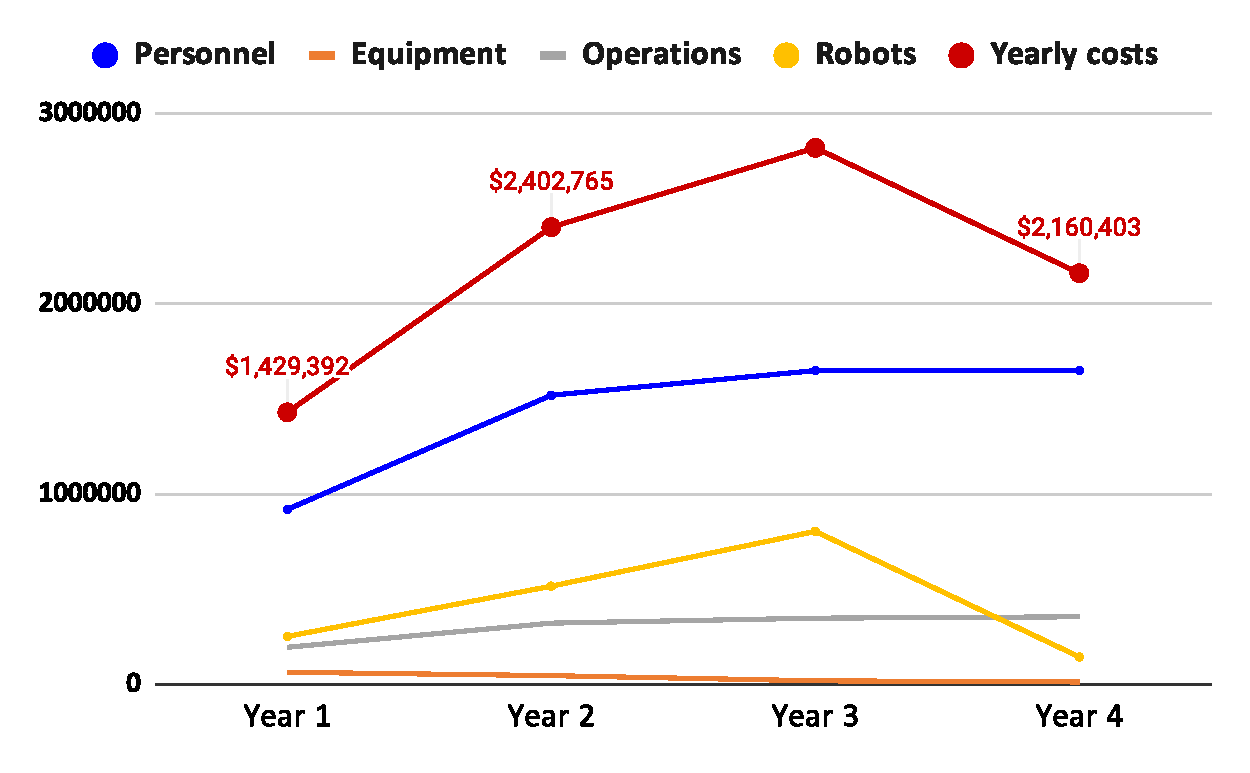
\includegraphics[scale=0.4]{fig/expenses.pdf}}
  \subfigure[]{\label{fig:exp-pie}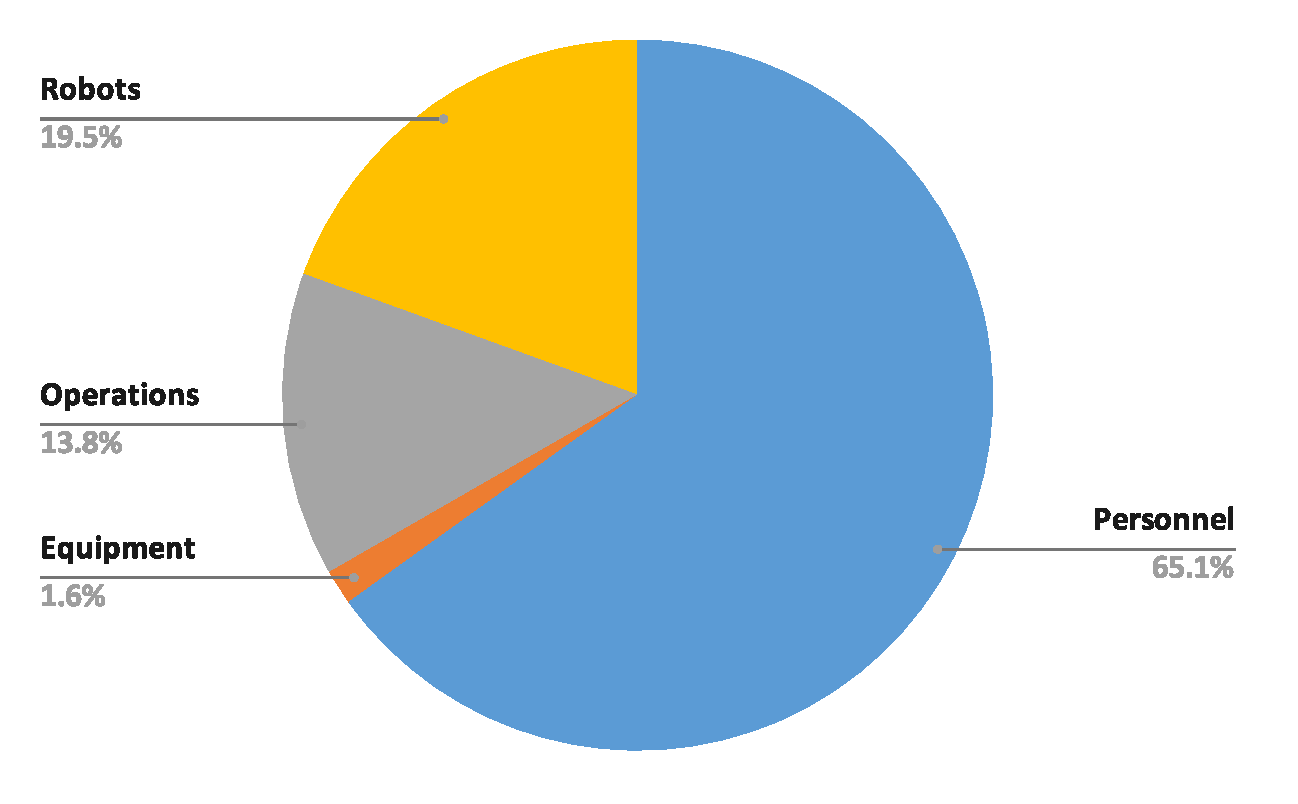
\includegraphics[scale=0.36]{fig/expenses-pie.pdf}}
  \caption{Budget needs and distribution for a 4-year project term:
    \subref{fig:expense} Total expenses related to personnel and
    equipment for a 4-year term; \subref{fig:exp-pie} Proportions of
    total budget for different uses (4-year averages).}
  \label{fig:costs}
  \vspace{-0.5cm}
\end{figure}

\subsection{Resources Needed}

The \pro team (see biographies below) comes ready with aerial, surface
and underwater vehicle platforms, together with the extensive suite of
communication software to provide coordinated observations in the
coastal ocean at the UPorto and SOCIB. With sensors measuring key
ocean variables, the focus of our effort will be in integrating
multiple data streams, increasing modeling skill with assimilated data
and adaptively targeting the in-situ vehicles to narrow the knowledge
gap of current oceanographic conditions. For this effort we will
continue to rely on existing remote sensing data products for
environmental assimilation. This in turn will provide a clear
consistent set of data products to provide actionable information to
policymakers on the ground, and society at large.

% comes ready with aerial, surface and underwater vehicle platforms,
% together with the extensive suite of communication software to provide
% coordinated observations in the coastal ocean at the \univ and
% \soce. With sensors measuring key ocean variables, the focus of our
% effort will be in integrating multiple data streams, increasing
% modelling skill with assimilated data and adaptively targeting the
% in-situ vehicles to narrow the knowledge gap of current oceanographic
% conditions. For this effort we will continue to rely on existing
% remote sensing data products for environmental assimilation. This in
% turn
% % We will integrate custom sensors keyed towards important ocean
% % variables integrated into a 'train' of \sml platforms.  Such a system
% % working synchronously with in-situ robots
% will provide a clear consistent set of data products to provide
% actionable information to policymakers on the ground, as also society
% in general.

We estimate the total project cost to be $\sim\$8.8$ Million over a
period of 4 years. As milestones are met in the first two years, and
the integrated software can be demonstrated on targeted use-cases,
\pro is likely to attract funding from public and private
sources. % Consequently, the project can also be funded in incremental
% steps:

% \begin{itemize}[noitemsep,topsep=0pt,parsep=0pt,partopsep=0pt]

% \item an initial focus on the software build, integration and test
%   with available robotic vehicles in small scale demonstrations $\sim
%   \$5$--$\$10$ Million for years 1 \& 2.

% \item acquisition of robotic vehicles, buoys, floats and a range of
%   sensors as payloads for these in-situ vehicles, their integration,
%   deployment and demonstration at increasingly larger spatial and
%   temporal scales for $\sim \$20$--$\$30$ Million in years 2 \& 3.

% \item acquisition of funds for a suitable at-scale design, build,
%   test, launch and operation of a \sml constellation with a range of
%   scientific payloads for biological and physical oceanographic
%   measurements for $\sim \$25$ Million in years 4 \& 5.

% \end{itemize}  

% Incremental build and evaluation of this concept can allow us to
% attract a wide range of public and private sponsors in the US and
% Europe.  Equally, we will consistently work with our collaborators in
% the Portuguese government to leverage expensive ship time for testing,
% and other potential in-kind contributions from Portuguese and Spanish
% resources.

% For a long-term operation and viability of this system, multiple
% outcomes can be envisioned. First, with the experience garnered in
% testing and fielding the system, a commercial spin-off of all or parts
% of the technology could be likely. If parts of the technology could be
% monetized and spun off to other companies, \pro can then hold the IP
% while continuing to work on research outcomes after the 4 year
% term. Second, the project can itself look for contracts from
% mega-cities and governments or their agencies to provide a
% software-as-a-service model and be able to subsist as a not-for-profit
% enterprise with unique expertise. Should other private or public
% funding sources be available, those would also be carefully evaluated
% to sustain operations and maintain an R\&D effort.

For a long-term operation and viability of this system, multiple
outcomes can be envisioned. First, with the experience garnered in
testing and fielding the system, a commercial spin-off of all or parts
of the technology could be likely. If parts of the technology could be
monetized and spun off to other companies, \pro can then hold the IP
while continuing to work on research outcomes after the 4-year
term. Second, the non-profit entity that will run the project, can
itself look for contracts from mega-cities and governments or their
agencies to provide a software-as-a-service model and be able to
subsist as a not-for-profit enterprise with unique expertise. Should
other private or public funding sources be available, those would also
be carefully evaluated to sustain operations and maintain an R\&D
effort.
